%!TEX root = ../report.tex
\documentclass[../report.tex]{subfiles}

\begin{document}
    \section{Introduction}
    % \label{sec:introduction}

    % This is a template for MAS R\&D projects, based on \emph{IEEETran}.
    % Here are some preliminaries about some common things you need to do to use the template:
    % \begin{itemize}
    %     \item Add your references to the file \emph{references.bib} and cite them as Mustermann and Smith \cite{referenceexample} (if there are more than three authors, cite as Mustermann et al. \cite{referenceexample}).
    %     \item Refer to sections as Sec. \ref{sec:introduction}.
    %     \item You can include figures as follows (note that the figure caption is below the figure).
    %     \begin{figure}[ht]
    %         \centering
    %         
\includegraphics[width=0.8\linewidth]{figures/b-it-logo.pdf}
    %         \caption{My caption}
    %         \label{fig:figureexample}
    %     \end{figure}
    %     Refer to figures as Fig. \ref{fig:figureexample}.
    %     \item You can add tables as follows (note that the table caption is above the table).
    %     \begin{table}[ht]
    %         \caption{My caption}
    %         \label{tab:tableexample}
    %         \begin{tabular}{M{0.45\linewidth} M{0.45\linewidth}}
    %             \hline
    %             \cellcolor{gray!10!white} Header 1 & \cellcolor{gray!10!white} Header 2 \\\hline
    %             Cell 1 & Cell 2 \\\hline
    %             Cell 3 & Cell 4 \\\hline
    %         \end{tabular}
    %     \end{table}
    %     Refer to tables as Tab. \ref{tab:tableexample}.
    %     \item You can add equations as follows.
    %     \begin{equation}
    %         f(x) = \frac{1}{\sigma\sqrt{2\pi}}e^{-\frac{1}{2}\left( \frac{x - \mu}{\sigma} \right)^2}
    %         \label{eq:equationexample}
    %     \end{equation}
    %     Refer to equations as Eq. \ref{eq:equationexample}.
    % \end{itemize}

    \subsection{Motivation}
    \label{sec:introduction:motivation}
Imagine standing inside a dense forest, looking at a vast expanse of trees, vegetation, and natural beauty. Now, imagine the challenge of understanding and analyzing the complex terrain hidden within that forest. This is the inspiration for this R\&D project. My mission is to develop a robust and efficient method to segment the forest terrain from the point-cloud data obtained through LiDAR technology. This will involve accurately identifying and excluding objects on the forest surface, such as tree stumps, tree trunks, and dense vegetation. In doing so, My team can gain valuable insight into the terrain and its characteristics, paving the way for effective forest management and planning.
{The forest terrain is rough and uneven, with different height-varying objects scattered throughout. This complexity makes it difficult to distinguish between the actual terrain and the objects on the forest floor. It requires advanced algorithms and techniques to accurately filter and process the LiDAR data, ensuring that the sensor captures only the relevant information. My goal is to develop such an algorithm.}

{To overcome these challenges, I am going to dive into the latest challenges and methods in LiDAR data analysis. I am also exploring various filtering, processing, and visualization techniques to make sense of the vast amount of data. I aim to automatically detect and segment the forest terrain without obstacles, providing a clear understanding of the forest's topography. This endeavor will significantly contribute to forest management, ecological research, and land-use planning by offering precise and actionable insights into the underlying terrain.}
    
    \subsection{Problem Statement}
    \label{sec:introduction:problem_statement}
    \begin{figure}[H]
        \centering
        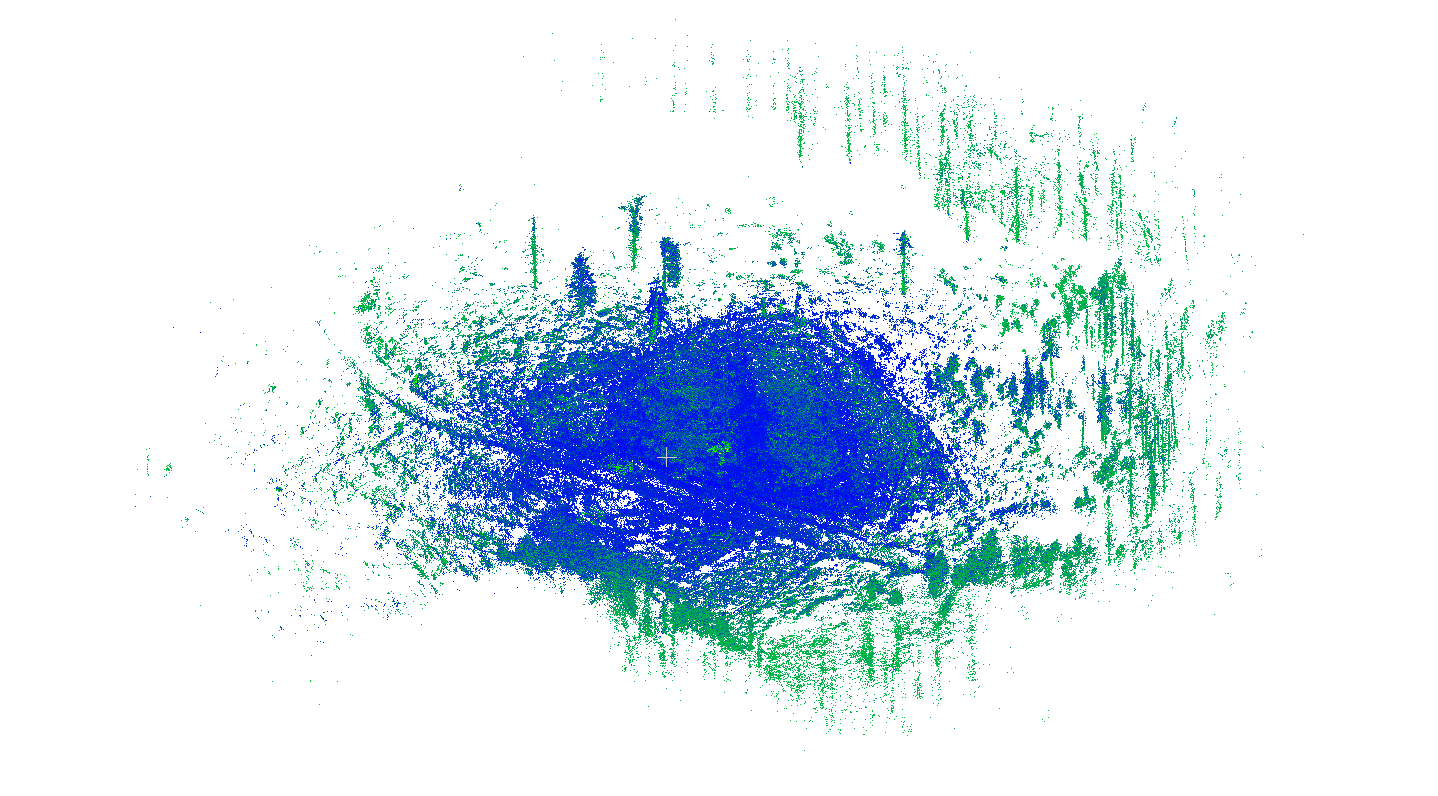
\includegraphics[width=0.4\textwidth]{rnd-project-report-main/figures/Original_data.png}
        \caption{Original LiDAR Data}
        \label{fig:raw_data}
    \end{figure}
    
The project addresses the challenge of accurately segmenting terrain from LiDAR point cloud data in complex forest environments. Raw LiDAR scans capture a dense collection of 3D points representing not just the ground but also a variety of objects, such as tree trunks, stumps, and dense vegetation. The primary problem lies in distinguishing the actual terrain from these overlying objects, given the ruggedness and heterogeneity of forest floors. Existing methods often struggle with transformation invariance, scalability, high computational demands, and the need for large labeled datasets, resulting in suboptimal segmentation and classification performance. This project aims to develop a potent and efficient classification system that can automatically clean, process, and segment LiDAR point cloud data to accurately identify and separate terrain from other objects, thereby enabling improved ecological analysis and forest management.
    \subsection{Proposed Approach}
    
    \label{sec:introduction:proposed_approach}
The project adopts a multi-stage, unsupervised learning pipeline for point cloud terrain segmentation, leveraging both classical and state-of-the-art machine learning techniques:
\subsubsection{Data Acquisition and Preprocessing}
Raw LiDAR point cloud data is collected, providing 3D coordinates for each scanned point. The data undergoes cleaning to remove outliers and normalization to standardize features, ensuring consistency and reliability for downstream analysis. The Open3D library is utilized for efficient point cloud processing.
\subsubsection{Feature Extraction}
Key geometric features—density, curvature, and height—are extracted from the cleaned data. These features are selected for their effectiveness in differentiating terrain from objects like tree trunks and stumps. Tools such as Open3D and PointNet are used for detailed feature analysis.\cite{Open3D_Library}\cite{PointNet}
\subsubsection{Unsupervised Clustering and Segmentation}
Clustering algorithms, including DBScan and hierarchical clustering, are applied to group points based on feature similarity. This step segments the point cloud into clusters corresponding to different physical entities within the terrain, such as ground, stumps, and trunks.\cite{DBSCAN}\cite{DBSCan_Grammarly}
\subsubsection{Cluster Classification}
Further refinement is achieved through K-Means clustering, categorizing the segmented clusters into distinct classes. Advanced methods like Cloth Simulation Filtering (CSF) for ground extraction and PointNet++ for deep feature learning are employed to enhance classification accuracy and scalability. PyTorch serves as the primary framework for implementing these models.\cite{ClothSF}\cite{PointNet++}
\subsubsection{Validation and Evaluation}
The effectiveness of the segmentation and classification is assessed using multiple validation metrics, including the silhouette coefficient, Davies-Bouldin index, and Calinski-Harabasz index. These metrics evaluate cluster cohesion and separation. Spatial validation ensures consistency across different regions, supporting practical ecological applications.\cite{Davies-Bouldin}\cite{Calinski}
This code pipeline is designed to overcome the limitations of existing methods by ensuring transformation invariance, reducing reliance on labeled data through unsupervised learning, promoting scalability via architecture-agnostic design, and optimizing performance for large-scale, real-world forest datasets. The outcome is a validated segmentation model that provides actionable insights for forest management, ecological research, and land-use planning.

\subsection{Conclusion}
This pipeline enables the training of models for the classification and part segmentation of tree trunks, stumps, and terrain using LiDAR data combined with clustering and deep learning techniques.


\end{document}
